\documentclass[letterpaper,12pt]{article}

\usepackage{times,amsmath,amsbsy,amssymb,amscd,mathrsfs}
%\usepackage{slashbox}\usepackage{graphicx,subfigure,epstopdf,wrapfig,chemarrow}

\usepackage{algorithm2e} 
\usepackage{multicol,multirow}
\usepackage{mathtools}
\usepackage[usenames,dvipsnames,svgnames,table]{xcolor}
\usepackage[all]{xy}
\usepackage{wrapfig}
\usepackage{tcolorbox}

%\usepackage[labelformat=simple]{subfig}
%\usepackage[hang,small,bf]{caption}

\usepackage{tikz,tikz-cd}
\usepackage[utf8]{inputenc}
\usepackage{pgfplots} 
\usepackage{pgfgantt}
\usepackage{pdflscape}
\pgfplotsset{compat=newest} 
\pgfplotsset{plot coordinates/math parser=false}
\newlength\fwidth

%\usepackage[notcite,notref]{showkeys}
\usepackage[numbered]{mcode}

\definecolor{myBlue}{rgb}{0.0,0.0,0.55}
%\definecolor{green}{rgb}{0.0,0.7,0.2}
\usepackage[pdftex,colorlinks=true,citecolor=myBlue,linkcolor=myBlue]{hyperref}

\usepackage[hyperpageref]{backref}

%\newcommand{\LC}[1]{\textcolor{cyan}{#1}}
\newcommand{\LC}[1]{\textcolor{red}{#1}}
\newcommand{\XH}[1]{\textcolor{cyan}{#1}}


\usepackage{comment,enumerate,multicol,xspace}

  \newcounter{mnote}
  \setcounter{mnote}{0}
  \newcommand{\mnote}[1]{\addtocounter{mnote}{1}
    \ensuremath{{}^{\bullet\arabic{mnote}}}
    \marginpar{\footnotesize\em\color{red}\ensuremath{\bullet\arabic{mnote}}#1}}
  \let\oldmarginpar\marginpar
    \renewcommand\marginpar[1]{\-\oldmarginpar[\raggedleft\footnotesize #1]%
    {\raggedright\footnotesize #1}}

%\usepackage[pdftex,dvipsnames]{xcolor}

%\usepackage{xargs} % Use more than one optional parameter in a new commands
%\usepackage[colorinlistoftodos,prependcaption,textsize=footnotesize]{todonotes}
%
%\newcounter{mycomment}
%\newcommand{\mycomment}[2][]{%
%% initials of the author (optional) + note in the margin
%\refstepcounter{mycomment}%
%{%
%\todo[linecolor=blue,backgroundcolor=blue!25,bordercolor=blue]{%
%\textbf{Comment [{\sc #1\themycomment}]:}\\#2}%
%}}
%
%\newcommandx{\change}[2][1=]
%{\todo[linecolor=OliveGreen,backgroundcolor=OliveGreen!25,bordercolor=OliveGreen,#1]{%
%{\sc Change}:\\#2}}
%
%\newcommandx{\improvement}[2][1=]
%{\todo[linecolor=Plum,backgroundcolor=Plum!25,bordercolor=Plum,#1]{%
%{\sc Improvement}:\\#2}}
%
%\newcommandx{\unsure}[2][1=]
%{\todo[linecolor=red,backgroundcolor=red!25,bordercolor=red,#1]{%
%{\sc Unsure}:\\ #2}}
%

% \newcommand{\mnote}[1]{}
\newcommand{\breakline}{
\begin{center}
------------------------------------------------------------------------------------------------------------
\end{center}
}
%\usepackage{geometry}
%%\usepackage{graphicx,pst-eps,epstopdf}
%\geometry{letterpaper, margin=1.5in}

\newtheorem{theorem}{Theorem}[section]
\newtheorem{lemma}[theorem]{Lemma}
\newtheorem{corollary}[theorem]{Corollary}
\newtheorem{proposition}[theorem]{Proposition}
\newtheorem{definition}[theorem]{Definition}
\newtheorem{example}[theorem]{Example}
\newtheorem{exercise}[theorem]{Exercise}
\newtheorem{question}[theorem]{Question}
\newtheorem{remark}[theorem]{Remark}
\newtheorem{alg}[theorem]{Algorithm}
%\newtheorem{answer}[proof]{Question}

\newcommand{\dx}{\,{\rm d}x}
\newcommand{\dd}{\,{\rm d}}
\newcommand{\deq}{\stackrel{\rm def}{=}}
\newcommand{\mbb}{\mathbb}
\newcommand{\mbf}{\bs}
\newcommand{\bs}{\boldsymbol}
\newcommand{\mcal}{\mathcal}
\newcommand{\mc}{\mcode}
\newcommand{\lla}{\langle}
\newcommand{\rra}{\rangle}
\newcommand{\supp}{\operatorname{supp}}
\newcommand{\range}{\operatorname{range}}
\newcommand{\PartSize}{\fontsize{0.85cm}{0.85cm}\selectfont} 
\newcommand{\mscr}{\mathscr}
\DeclarePairedDelimiter\ceil{\lceil}{\rceil}
\DeclarePairedDelimiter\floor{\lfloor}{\rfloor}

%\newcommand{\span}{\rm span}
\newcommand{\red}{\color{red}}
\newcommand{\green}{\color{green}}
\newcommand{\blue}{\color{blue}}
\newcommand{\gray}{\color{gray}}

%\DeclareMathOperator*{\curl}{curl}
\DeclareMathOperator*{\img}{img}
\DeclareMathOperator*{\spa}{span}
\DeclareMathOperator*{\diag}{diag}
\newcommand{\curl}{{\rm curl\,}}
\renewcommand{\div}{\operatorname{div}}
%\renewcommand{\grad}{\operatorname{grad}}
\newcommand{\grad}{{\rm grad\,}}
%\DeclareMathOperator*{\tr}{tr}
\DeclareMathOperator*{\rot}{rot}
\DeclareMathOperator*{\var}{Var}
\DeclareMathOperator{\rank}{rank}
\DeclareMathOperator{\dist}{dist}
%\DeclareMathOperator{\span}{span}
\newcommand{\tr}{\operatorname{tr}}
\newcommand{\dev}{\operatorname{dev}}
\newcommand{\sym}{\operatorname{sym}}
\newcommand{\skw}{\operatorname{skw}}
\newcommand{\spn}{\operatorname{spn}}
\newcommand{\mspn}{\operatorname{mspn}}
\newcommand{\vspn}{\operatorname{vspn}}
\newcommand{\mskw}{\operatorname{mskw}}
\newcommand{\vskw}{\operatorname{vskw}}
\newcommand{\defm}{\operatorname{def}}
\newcommand{\hess}{\operatorname{hess}}
\newcommand{\inc}{\operatorname{inc}}
\newcommand{\dex}{\operatorname{dex}}

\newcommand{\step}[1]{\noindent\raisebox{1.5pt}[10pt][0pt]{\tiny\framebox{$#1$}}\xspace}

%\usepackage[margins]{trackchanges}
%\renewcommand{\initialsOne}{chen}

\newcommand{\norm}[1]{\left\Vert#1\right\Vert}
\newcommand{\snorm}[1]{\left\vert#1\right\vert}
\newcommand{\vertiii}[1]{{\left\vert\kern-0.25ex\left\vert\kern-0.25ex\left\vert #1 
    \right\vert\kern-0.25ex\right\vert\kern-0.25ex\right\vert}}


\title{子空间矫正法与辅助空间法}
\author{陈春雨}
\date{}

\begin{document}
\maketitle
在偏微分方程数值解方法中,算子方程:
\begin{equation}
    Au = f,
\end{equation}
的求解是一个重要的基础问题。这里 $A$ 是一个线性算子,$u$ 是未知函数,$f$
是已知函数。
当 $\mathbb{V} \equiv \mathbb{R}^d$ 
是一个 Hilbert 空间,$A : \mathbb{V} \to \mathbb{V}$
是一个对称正定算子时,求解方法有很多,例如共轭梯度法、GMRES
方法等,
在本章中,我们将讨论由 Xu 等人发展起来的子空间修正方法和辅助空间方法,
本文档的内容参考了 Long Chen 的课程讲义[].

\section{空间分解与子空间修正方法}

将空间 $\mathbb{V}$ 分解为子空间的和,相应地将问题 (1) 分解为若干规模较小的问题,这些子问题相对较易求解。

令 $\{\mathbb{V}_i\}_{i=1}^J$ 是 $\mathbb{V}$ 的一组子空间,
若 $\mathbb{V} = \sum_{i=0}^{J} \mathbb{V}_i$,则称 $\{\mathbb{V}_i\}_{i=1}^J$
为 $\mathbb{V}$ 的\textbf{空间分解}。根据定义,对于任意 $v \in V$,我们可以写成:
$$
v = \sum_{i=1}^J v_i, \quad v_i \in \mathbb{V}_i, \; i = 1, \dots, J.
$$
由于 $\sum_{i=1}^J \mathbb{V}_i$ 不一定是直和,因此该分解不唯一。
为了下面的讨论,我们给出如下引理:
\begin{lemma}
    \label{lem:operatoreq}
    $U$ 和 $V$ 是 Hilbert 空间,
    若 $P, Q$ 是两个 $U \to V$ 的线性算子,那么 $P = Q$ 当且仅当
    \begin{equation}
        (P u, v) = (Q u, v) \quad \forall u \in U, v \in V.
    \end{equation}
\end{lemma}
现在引入以下算子:
\begin{itemize}
    \item $I_i: \mathbb{V}_i \to \mathbb{V}$ 自然嵌入;
    \item $Q_i: \mathbb{V} \to \mathbb{V}_i$ 投影算子,相对于内积 $(\cdot, \cdot)$;
    \item $P_i: \mathbb{V} \to \mathbb{V}_i$ 投影算子,相对于内积 $A(\cdot, \cdot)$;
    \item $A_i: \mathbb{V}_i \to \mathbb{V}_i$ 是 $A$ 在子空间 $\mathbb{V}_i$
        上的限制;
    \item $R_i: \mathbb{V} \to \mathbb{V}_i$ 是 $A^{-1}_i$ 的一个近似,
        也称为\textbf{光滑算子}; 
    \item $T_i: \mathbb{V} \to \mathbb{V}_i$: 
        $T_i = R_i A P_i = R_i A_i P_i$;
\end{itemize}
我们探讨这些算子之间的关系。
$I_i$ 只能作用于 $\mathbb{\mathbb{V}}_i$ 上。
$Q_i$ 和 $P_i$ 可以作用于 $\mathbb{V}$ 上,且有 
\begin{align}
(Q_i u, v_i) & = (u, v_i) \quad
\forall v_i \in \mathbb{V}_i, u \in \mathbb{V} 
\label{eq:Q}\\
(P_i u, A v_i) & = (u, A v_i) \quad
\forall v_i \in \mathbb{V}_i, u \in \mathbb{V} \label{eq:P}
\end{align}
由 \eqref{eq:Q} 可知 
$$
\begin{aligned}
(u, Q_i^T v_i) & = (Q_i u, v_i) = (u, v_i) \quad u \in \mathbb{V}, v_i \in
\mathbb{V}_i,
\end{aligned}
$$
$Q_i^T$ 和 $I_i$ 都是 $\mathbb{V}_i$ 到 $\mathbb{V}$ 的线性算子,所以根据引理
\ref{lem:operatoreq},$Q_i^T = I_i$。
类似的由 \eqref{eq:P} 可知
$$
\begin{aligned}
    (P_i u, A v_i) & = (P_i u, Q_i A v_i) =
    (A Q_i^TP_i u, v_i) = (Q_i A Q_i^T P_i u, v_i) \quad u \in
    \mathbb{V}, v_i \in \mathbb{V}_i, \\
    (u, A v_i) & = (A u, v_i) = (Q_i A u, v_i) \quad u \in \mathbb{V}, v_i \in
    \mathbb{V}_i.
\end{aligned}
$$
因为 $Q_iA$ 和 $Q_iAQ_i^TP_i$ 都是 $\mathbb{V}_i$ 到 $\mathbb{V}_i$
的线性算子,所以类似的根据引理 \ref{lem:operatoreq},$Q_iA = Q_iAQ_i^TP_i$。
另外 $A_i$ 是 $A$ 在 $\mathbb{V}_i$ 上的限制, $A_iv_i = Q_i A v_i = 
Q_iAI_i v_i$ 即 $A_i$ 作用的结果是 $A$ 作用后再正交投影到 $\mathbb{V}_i$ 上:
$A_i = Q_i AI_i = I_i^TAI_i = Q_i A Q_i^T$。所以:
$$
A_iP_i = Q_iA.
$$
当把 $P_i$ 和 $Q_i$ 限制在 $\mathbb{V}_i$ 上时,$P_i$ 和 $Q_i$ 都是恒等算子即:
$$
P_i I_i = I_i, \quad Q_i I_i = I_i.
$$
所以 $P_i$ 和 $Q_i$ 都是幂等算子。

在实际应用中,$I_i$ 称为\emph{延拓算子},其矩阵是 $\mathbb{V}_i$ 到 $\mathbb{V}$
的基向量延拓矩阵。$Q_i = I_i^T$ 是\emph{限制算子},即 $\mathbb{V}$ 到 $\mathbb{V}_i$
的限制函数。

我们有如下交换图:
\[
\begin{array}{ccc}
\mathbb{V} & \xrightarrow{A} & \mathbb{V} \\
\downarrow P_i & & \downarrow Q_i \\
\mathbb{V}_i & \xrightarrow{A_i} & \mathbb{V}_i \\
\end{array}
\]

{\color{red} 下面的需要修改}


一致的记号为:将 $R_i$ 用于平滑器的迭代器,而 $B$ 是原问题迭代器的记号。但我们将保留 $B$ 表示原问题的迭代器。

我们来看看算子 $T_i = R_i Q_i A P_i$,当 $P_i = I_{\mathbb{V}_i}$(即恒等嵌入)时,投影 $P_i$ 是恒等映射,此时 $T_i = R_i A_i$。当 $T_i$ 被限制在 $\mathbb{V}_i$ 上时,我们记为 $T_i|_{\mathbb{V}_i} = (T_i|_{\mathbb{V}_i})^{-1}$。$T_i$ 的作用为:

\[
(T_i u_i, v_i)_A = (R_i^{-1} u_i, v_i), \quad \forall v_i \in \mathbb{V}_i.
\]

\section{子空间修正方法描述}

我们现在描述子空间修正方法。为了便于讨论,设 $r = Q_i^T v$ 表示残差在子空间上的限制。我们将求解子空间上的残差方程 $A_i e_i = r$,其解为:

\[
e_i = R_i r = R_i Q_i^T v.
\]

子空间修正被组装用于在空间 $\mathbb{V}$ 中给出修正,因此称为“子空间修正方法”。

基本上,有两种组装子空间修正的方法:

\subsection{并行子空间修正(PSC)}

此方法是对每个子空间上的修正并行进行。在算子形式下为:

\begin{equation}
u_{k+1} = u_k + B_0 (f - A u_k) = u_k + \sum_{i=1}^J R_i Q_i^T (f - A u_k),
\end{equation}

其中

\[
B_0 := \sum_{i=1}^J R_i Q_i^T.
\]

\subsection{逐次子空间修正(SSC)}

子空间修正为:

\[
e_i = R_i Q_i^T (f - A u_k),
\]

并依次对每个子空间修正。此方法以逐次方式进行。在算子形式下为:

\begin{equation}
v^0 = u_k, \quad v^i = v^{i-1} + R_i Q_i^T (f - A v^{i-1}), \quad i = 1, \dots, J,
\end{equation}

\begin{equation}
u_{k+1} = v^J.
\end{equation}

该迭代器 $B_{SSC}$ 不容易公式化。

\begin{figure}[htbp]
    \centering
    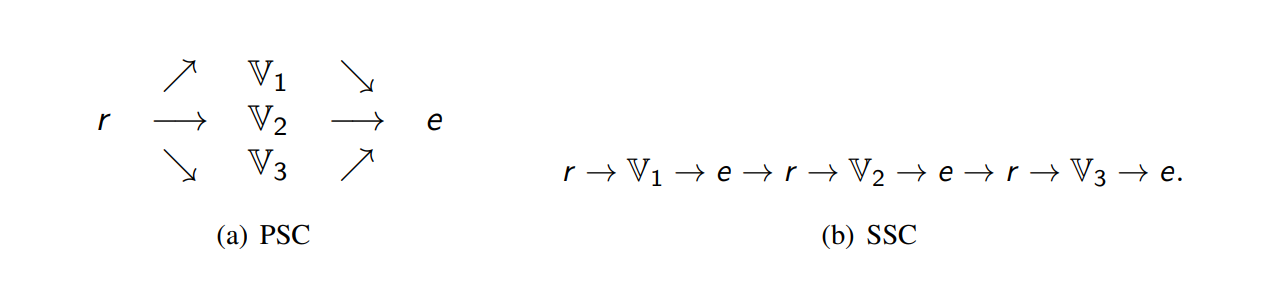
\includegraphics[width=1.0\textwidth]{./figure/psc_and_ssc.png}
    \caption{PSC 与 SSC 方法示意图:(a) PSC;(b) SSC。箭头表示从 $r \to \mathbb{V}_i \to e \to \cdots \to \mathbb{V}_3 \to e$ 的修正流程。}
\end{figure}

对于 PSC 和 SSC 方法,我们有以下误差估计:

\begin{itemize}
    \item \textbf{并行子空间校正 (PSC)}: \[ u-u_{k+1}=\left[I-\sum_{i=1}^{J}T_{i}\right](u-u_{k}); \]
    
    \item \textbf{逐次子空间校正 (SSC)}: \[ u-u_{k+1}=\prod_{i=1}^{J}(I-T_{i})\bigg{]}(u-u_{k}). \]
\end{itemize}

因此PSC也被称为\textbf{加法型方法},而SSC被称为\textbf{乘法型方法}。在符号$\prod_{i=1}^{J}a_{i}$中,我们假定存在从$i=1$到$N$的内置顺序,即$\prod_{i=1}^{J}a_{i}=a_{0}a_{1}\ldots a_{N}$。

我们以下列算法形式展示PSC和SSC,强调其是求解残差方程的过程——给定残差$r$,返回修正量$e$。PSC或SSC的一次迭代可用作FCC中的预条件子。

\begin{verbatim}
function e = PSC(r)
% 用PSC方法求解残差方程Ae=r
e = 0;
for i = 1:J
    r_i = I_i * r;          % 将残差限制到子空间
    e_i = R_i \ r_i;        % 在子空间中求解残差方程
    e = e + I_i^T * e_i;    % 将修正量延拓到大空间
end

function e = SSC(r)
% 用SSC方法求解残差方程Ae=r
e = 0;
for i = 1:J
    r_i = I_i * r;          % 将残差限制到子空间
    e_i = R_i \ r_i;        % 在子空间中求解残差方程
    e = e + I_i^T * e_i;    % 将修正量延拓到大空间
    r = r - A * e;          % 更新残差
end
\end{verbatim}

比较上述PSC和SSC函数可见:在SSC中,每次子空间校正后会更新残差,而PSC则不会。在收敛速度方面,SSC更优;另一方面,PSC具有天然的并行性,而SSC本质上是串行方法。

\subsection{例}
考虑矩阵方程
\[ Au=f, \]
其中$A$是$N\times N$对称正定矩阵。取$\mathbb{R}^{N}=\sum_{i=1}^{N}\text{span}\{e_{i}\}$的平凡分解($\{e_{i},i=1,\ldots,N\}$是$\mathbb{R}^{N}$的标准基),则:

\begin{itemize}
    \item 当$R_{i}=\omega I$时,PSC即为Richardson方法;
    \item 当$R_{i}=A_{i}^{-1}$时,PSC即为Jacobi方法;
    \item 当$R_{i}=A_{i}^{-1}$时,SSC即为Gauss-Seidel方法。
\end{itemize}

后续我们还将把PSC视为乘积空间大系统的Jacobi方法,SSC视为同一系统的Gauss-Seidel方法。

\section{辅助空间方法}

本节介绍Nepomnyaschikh的虚拟空间方法[4]和Xu的辅助空间方法[6]的变体,内容组织参考[1]。

设$\mathbb{\mathbb{V}}$和$\tilde{\mathbb{\mathbb{V}}}$为两个Hilbert空间,$\Pi:\tilde{\mathbb{\mathbb{V}}}\to\mathbb{\mathbb{V}}$为满射映射。在默认内积下定义$\Pi$的伴随算子$\Pi^{\tau}:\mathbb{\mathbb{V}}\to\tilde{\mathbb{\mathbb{V}}}$满足:
\[ (\Pi^{\tau}u,\tilde{v}) = (u,\Pi\tilde{v}) \quad \forall u\in\mathbb{\mathbb{V}}, \tilde{v}\in\tilde{\mathbb{\mathbb{V}}} \]
此处为简化符号,$\mathbb{\mathbb{V}}$和$\tilde{\mathbb{\mathbb{V}}}$的内积均用$(\cdot,\cdot)$表示。由于$\Pi$是满射,其转置$\Pi^{\tau}$是单射。

给定SPD算子$A:\mathbb{\mathbb{V}}\to\mathbb{\mathbb{V}}$,定义$A$的提升算子$\tilde{A}=\Pi^{\tau}A\Pi:\tilde{\mathbb{\mathbb{V}}}\to\tilde{\mathbb{\mathbb{V}}}$。为构造$A^{-1}$的良好近似,可先构造$\tilde{A}^{-1}$的近似。设$\tilde{B}:\tilde{\mathbb{\mathbb{V}}}\to\tilde{\mathbb{\mathbb{V}}}$为SPD算子,定义$B:=\Pi\tilde{B}\Pi^{\tau}:\mathbb{\mathbb{V}}\to\mathbb{\mathbb{V}}$,下文将证明其仍保持SPD性质。关系总结如下:

\[
\begin{array}{ccc}
\tilde{\mathbb{\mathbb{V}}} & \stackrel{\tilde{A}}{\longleftarrow} & \tilde{\mathbb{\mathbb{V}}} \\
\Pi \uparrow & & \downarrow \Pi^{\tau} \\
\mathbb{\mathbb{V}} & \stackrel{A}{\longleftarrow} & \mathbb{\mathbb{V}}
\end{array}
\]

\begin{theorem}[2.1]
设$\tilde{\mathbb{\mathbb{V}}}$和$\mathbb{\mathbb{V}}$为Hilbert空间,$\Pi:\tilde{\mathbb{\mathbb{V}}}\to\mathbb{\mathbb{V}}$为满射,$\tilde{B}:\tilde{\mathbb{\mathbb{V}}}\to\tilde{\mathbb{\mathbb{V}}}$为对称正定算子。则$B:=\Pi\tilde{B}\Pi^{\tau}:\mathbb{\mathbb{V}}\to\mathbb{\mathbb{V}}$也是对称正定的,且满足:
\[ (B^{-1}v,v) = \inf_{\Pi\tilde{v}=v} (\tilde{B}^{-1}\tilde{v},\tilde{v}) \]
\end{theorem}

\begin{proof}
采用Xu和Zikatanov[9](引理2.4)的证明方法。

显然$B$对称半正定。由于$\tilde{B}$SPD且$\Pi^{\tau}$单射,$(Bv,v)=(\tilde{B}\Pi^{\tau}v,\Pi^{\tau}v)=0$蕴含$\Pi^{\tau}v=0$,从而$v=0$,故$B$正定。

令$\tilde{v}^{*}=\tilde{B}\Pi^{\tau}B^{-1}v$,则$\Pi\tilde{v}^{*}=v$。对任意$\tilde{w}\in\tilde{\mathbb{\mathbb{V}}}$有:
\[ (\tilde{B}^{-1}\tilde{v}^{*},\tilde{w}) = (\Pi^{\tau}B^{-1}v,\tilde{w}) = (B^{-1}v,\Pi\tilde{w}) \]
特别地:
\[ (\tilde{B}^{-1}\tilde{v}^{*},\tilde{v}^{*}) = (B^{-1}v,\Pi\tilde{v}^{*}) = (B^{-1}v,v) \]

对任意$\tilde{v}\in\tilde{\mathbb{\mathbb{V}}}$,记$v=\Pi\tilde{v}$,可分解为$\tilde{v}=\tilde{v}^{*}+\tilde{w}$其中$\Pi\tilde{w}=0$,则:
\[
\inf_{\Pi\tilde{v}=v} (\tilde{B}^{-1}\tilde{v},\tilde{v}) = \inf_{\Pi\tilde{w}=0} [ (\tilde{B}^{-1}\tilde{v}^{*},\tilde{v}^{*}) + 2(\tilde{B}^{-1}\tilde{v}^{*},\tilde{w}) + (\tilde{B}^{-1}\tilde{w},\tilde{w}) ] = (B^{-1}v,v)
\]
\end{proof}

对称正定算子$B$可作为预条件子用于PCC方法求解$Au=f$。为估计条件数$\kappa(BA)$,只需比较$B^{-1}$与$A$:

\begin{lemma}[2.2]
对两个SPD算子$A$和$B$,若满足$c_{0}(Av,v) \leq (B^{-1}v,v) \leq c_{1}(Av,v)$对所有$v\in\mathbb{\mathbb{V}}$成立,则$\kappa(BA) \leq c_{1}/c_{0}$。
\end{lemma}

\begin{proof}
注意到$BA$关于$A$对称,因此
\[
\lambda_{\min}(BA) = \lambda_{\max}((BA)^{-1}) = \sup_{u \in \mathbb{V}(A)} \frac{((BA)^{-1}u, u)_A}{(u, u)_A} = \sup_{u \in \mathbb{V}(A)} \frac{(B^{-1}u, u)}{(Au, u)}.
\]
故$(B^{-1}v, v) \leq c_1(Av, v)$蕴含$\lambda_{\min}(BA) \geq c_1^{-1}$;同理$(B^{-1}v, v) \geq c_0(Av, v)$蕴含$\lambda_{\max}(BA) \leq c_0^{-1}$,由此可得$\kappa(BA)$的估计。
\end{proof}

\begin{theorem}[2.3]
设$\tilde{\mathbb{V}}$和$\mathbb{V}$为Hilbert空间,$\Pi:\tilde{\mathbb{V}}\to \mathbb{V}$为满射,$\tilde{B}:\tilde{\mathbb{V}}\to\tilde{\mathbb{V}}$对称正定且$B=\Pi\tilde{B}\Pi^\tau$。若对所有$v\in \mathbb{V}$满足
\[
c_0(Av, v) \leq \inf_{\Pi\tilde{v}=v} (\tilde{B}^{-1}\tilde{v}, \tilde{v}) \leq c_1(Av, v),
\]
则
\[
\kappa(BA) \leq c_1/c_0.
\]
\end{theorem}

\begin{remark}[2.4]
文献中(如[4]的虚拟空间引理),条件(6)通常分解为:
\begin{enumerate}
    \item 对任意$v\in \mathbb{V}$,存在$\tilde{v}\in\tilde{\mathbb{V}}$使得$\Pi\tilde{v}=v$且$\|\tilde{v}\|_{\tilde{B}^{-1}}^2 \leq c_1 \|v\|_A^2$;
    \item 对任意$\tilde{v}\in\tilde{\mathbb{V}}$,$\|\Pi\tilde{v}\|_A^2 \leq c_0^{-1}\|\tilde{v}\|_{\tilde{B}}^2$。
\end{enumerate}
\end{remark}

\subsection{乘积型辅助空间}
给定空间分解$\tilde{\mathbb{V}}=\sum_{i=1}^J \mathbb{V}_i$,构造乘积型辅助空间$\tilde{\mathbb{V}}=\mathbb{V}_0\times \mathbb{V}_1\times\cdots\times \mathbb{V}_J$,其内积定义为$(\tilde{u},\tilde{v}):=\sum_{i=0}^J(u_i,v_i)$。定义$\Pi:\tilde{\mathbb{V}}\to \mathbb{V}$为$\Pi\tilde{u}=\sum_{i=0}^J u_i$。若将$\tilde{u}=(u_0,\ldots,u_J)$视为列向量,则$\Pi=[I_0,I_1,\ldots,I_J]$。由于$\tilde{\mathbb{V}}=\sum_{i=0}^J \mathbb{V}_i$,$\Pi$是满射。

令$\tilde{A}=\Pi^\tau A\Pi$,$\tilde{f}=\Pi^\tau f$。若$\tilde{u}$满足$\tilde{A}\tilde{u}=\tilde{f}$,两边同乘$\Pi$可验证$u=\Pi\tilde{u}$是$Au=f$的解。

\subsubsection{PSC与SSC的推导}
通过经典迭代法求解$\tilde{A}\tilde{u}=\tilde{f}$可得PSC和SSC方法。设$R_i:\mathbb{V}_i\to \mathbb{V}_i$为非奇异算子(常称为光滑子,近似$A_i^{-1}$),定义分块对角算子矩阵$R=\operatorname{diag}(R_0,R_1,\ldots,R_J):\tilde{\mathbb{V}}\to\tilde{\mathbb{V}}$。

直接计算可得$\tilde{A}_{ij}=Q_iAQ_j=A_iP_j$,其中$\tilde{A}_{ii}=A_i$。对称算子$\tilde{A}$可能有非平凡核$\ker(\Pi)$,但其对角块总非奇异。将$\tilde{A}$分解为$D+L+U$,其中$D=\operatorname{diag}(A_0,\ldots,A_J)$,$L$和$U$分别为下三角和上三角算子矩阵且$L^\tau=U$。

考虑迭代格式
\[
\tilde{u}_{k+1} = \tilde{u}_k + R(\tilde{f} - \tilde{A}\tilde{u}_k).
\]
令$u_k=\Pi\tilde{u}_k$,对(7)式应用$\Pi$并注意到$\tilde{f}=\Pi^\tau f$和$\tilde{A}\tilde{u}_k=\Pi^\tau Au_k$,可得PSC方法:
\[
u_{k+1} = u_k + \sum_{i=0}^J R_i Q_i(f - Au_k).
\]

乘法型方法更为精巧。参照[3],可将求解$Au=f$的SSC视为$\tilde{A}\tilde{u}=\tilde{f}$的高斯-赛德尔型方法。

\begin{lemma}[3.1]
设$A = D + L + U$且$B = (R^{-1} + L)^{-1}$,则采用局部求解器$R_i$求解$Au=f$的SSC方法等价于以下高斯-赛德尔型迭代:
\[ u_{k+1} = u_k + B(f - Au_k). \]
\end{lemma}

\begin{proof}
对(8)式左乘$R^{-1} + L$并整理项可得:
\[ R^{-1}u_{k+1} = R^{-1}u_k + f - Lu_{k+1} - (D + U)u_k. \]
再左乘$R$得到:
\[ u_{k+1} = u_k + R \left( f - Lu_{k+1} - (D + U)u_k \right), \]
其分量形式为($i=1,\ldots,J$):
\[
\begin{aligned}
u^{i}_{k+1} &= u^{i}_k + R_i \left( f - \sum_{j=1}^{i-1} A_{ij}u^{j}_{k+1} - \sum_{j=i}^{J} A_{ij}u^{j}_k \right) \\
&= u^{i}_k + R_i Q_i \left( f - A\sum_{j=1}^{i-1} u^{j}_{k+1} - A\sum_{j=i}^{J} u^{j}_k \right).
\end{aligned}
\]

定义动态更新:
\[
v^{i} = \Pi \left( u^{1}_{k+1}, \ldots, u^{i}_{k+1}, u^{i+1}_k, \ldots, u^{J}_k \right) = \sum_{j=1}^{i} u^{j}_{k+1} + \sum_{j=i+1}^{J} u^{j}_k.
\]
注意到$v^{i} - v^{i-1} = u^{i}_{k+1} - u^{i}_k$,则对$i=1,\ldots,J+1$有:
\[
v^{i} = v^{i-1} + R_i Q_i (f - Av^{i-1}),
\]
这正是子空间$\mathbb{V}_i$中的修正形式(参见式(4))。
\end{proof}

对于SSC方法,每个子空间问题的算子形式为$v^{i+1} = v^i + R_i(f - Av^i)$,但难以直接写出整个空间$\mathbb{V}$的迭代算子。定义误差算子$B_m$满足:
\[
I - B_m A = (I - R_J Q_J A) \cdots (I - R_0 Q_0 A).
\]

通过辅助空间方法可推导$B_m$的表达式。设$B_m = (R^{-1} + L)^{-1}$,其对称化版本为:
\begin{equation}
\overline{B}_m = B_m + B_m^\tau - B_m^\tau A B_m = B_m^\tau (B_m^{-1} + B_m^{-\tau} - A) B_m.
\end{equation}

\begin{lemma}[3.2]
对SSC方法有:
\[
B_m = \Pi \mathcal{B}_m \Pi^\tau \quad \text{且} \quad \overline{B}_m = \Pi \overline{\mathcal{B}}_m \Pi^\tau.
\]
\end{lemma}
\begin{proof}
令$u_k = \Pi \mathbf{u}_k$,对(8)式应用$\Pi$并注意到:
\[
f = \Pi^\tau f, \quad \text{且} \quad Au_k = \Pi^\tau A u_k,
\]
则得到:
\[
u_{k+1} = u_k + \Pi \mathcal{B}_m \Pi^\tau (f - Au_k).
\]
$\overline{B}_m$的表达式可通过类似计算得到。
\end{proof}

\end{document}
